
\documentclass[12pt]{article}
\usepackage{amsmath}
\DeclareMathOperator*{\argmin}{arg\,min} % thin space, limits underneath in displays
\DeclareMathOperator*{\argmax}{arg\,max} % thin space, limits underneath in displays
\newtheorem{thm}{Theorem}
\usepackage{amssymb}
\usepackage{amsfonts}
\usepackage{mathrsfs}
\usepackage{bm}
\usepackage{indentfirst}
\setlength{\parindent}{0em}
\usepackage[margin=1in]{geometry}
\usepackage{graphicx}
\usepackage{setspace}
\doublespacing
\usepackage[flushleft]{threeparttable}
\usepackage{booktabs,caption}
\usepackage{float}
\usepackage{graphicx}
\usepackage[sort,comma]{natbib}

\usepackage{import}
\usepackage{xifthen}
\usepackage{pdfpages}
\usepackage{transparent}

\newcommand{\incfig}[1]{%
\def\svgwidth{\columnwidth}
\import{./figures/}{#1.pdf_tex}
}




\title{}
\author{}
\date{}


\begin{document}
\maketitle
\section{Three statistics}
{\textbf {GDP:}}\\
Gross domestic product, or GDP, tells us the nation’s total income and the total 
expenditure on its output of goods and services.

{\textbf {CPI:}}\\
The consumer price index, or CPI, measures the level of prices. 

{\textbf {Unemployment rate:}}\\
The unemployment rate tells us the fraction of workers who are unemployed. 



\subsection{GDP}
There are two ways to view this statistic. 
One way to view GDP is as the total income of everyone in the
economy; another way is as the total expenditure on the economy’s output of goods 
and services. From either viewpoint, it is clear why GDP is a gauge of economic 
performance. How can GDP measure both the economy’s income and its expenditure on output?
It can do so because these two quantities are really the same: for the economy as 
a whole, income must equal expenditure. That fact, in turn, follows from an even more
fundamental one: because every transaction has a buyer and a seller,
every dollar of expenditure by a buyer must become a dollar of income to a seller. 
When Jack paints Jill’s house for \$10,000, that \$10,000 is income to Jack and 
expenditure by Jill. The transaction contributes \$10,000 to GDP, regardless of whether 
we are adding up all income or all expenditure.



\subsubsection{Two ways to compute GDP}

\begin{figure}[H]
\center{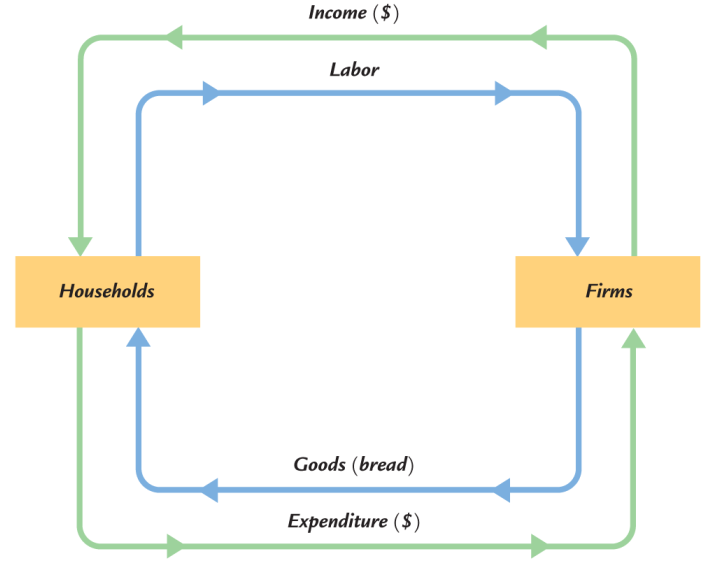
\includegraphics[scale =.5 ]  {figures/income_expenditure_circle_gdp.png}}
\end{figure}
{\textbf {1: Seller}}\\
We can compute it in two ways. GDP is the total income from the production of bread,
which equals the sum of wages and profit — the top half of the circula  flow of dollars.
(wage + profit = firm's income) 

{\textbf {2: Buyer}}\\
GDP is also the total expenditure on purchases of bread — the bottom half of the 
circular flow of dollars. To compute GDP, we can look at either the flow of dollars
from firms to households or the flow of dollars from households to firms.


{\textbf {These two ways of computing GDP must be equal because the expenditure of
buyers on products is income to the sellers of those products.}}


\subsubsection{Rules for computing GDP}
1. Values = price * quantity

2. Transfer is not part of GDP: Firm A produces and sells product for \$2, this is part
of the GDP. But if a collector sell a card to another collector for \$2, this is NOT
part of GDP. It is a transfer of an asset, not an addition to national income.


3. Inventory:\\
When a firm increases its inventory of goods, this investment in inventory is counted as
expenditure by the firm owners. Thus, production for inventory increases GDP just as much
as does production for final sale.

A sale out of inventory, however, combines positive spending (the purchase) and negative
spending (inventory disinvestment), so it does not affect GDP. This treatment of inventor
ies ensures that GDP reflects the economy’s current production of goods and services.


4. Intermediate goods:\\
Suppose a cattle rancher sells one-quarter pound of meat to McDonald’s for \$1, and 
then McDonald’s sells you a hamburger for \$3. 
GDP includes only the value of final goods. Thus, the hamburger is included in GDP, 
but the meat is not: GDP increases by \$3, not by \$4.
The reason is that the value of intermediate goods is already included as part of the 
market price of the final goods in which they are used.

Or we can calculate the value added. \$1 added for meat, and 3-1 = \$2 added for 
hamburger. Hence, total added value = 1+2 = 3.


5. Imputations:\\
Not all goods and services are sold in the mkt. Hence not all products have prices.
For these goods, we need to estimate the imputed value.

{\textbf {Case1: Housing}}\\
Renter pay rents to house owner. There's a expenditure for renter and a income for 
house owner. So this is counted as part of GDP. However, for those who live in their
own house, they also enjoy the service of housing, GDP includes the ``rent" they
pay to themselves. The department of commerce estimates the mkt rent. This imputed
value will be included in both houseowner's expenditure and income.


{\textbf {Case2:Gov't Services}}\\
Police officers, firefighters, and senators provide services to the public, but do not
have market price. The national accounts include these to services using their cost
e.g., the wage.

{\textbf {Not included:}}\\
Rent on cars, lawn mowers, jewelry, and other durable goods owned by households.
Yet the value of these rental services is left out of GDP.

Some of the output of the economy is produced and consumed at home and never enters the 
marketplace. They are out of the GDP, for example, home-made food.

No imputation is made for the value of goods and services sold in the 
{\textbf {underground economy}}.


{\textbf {NOTE:}}\\
Because the imputations necessary for computing GDP are only approximate, and because the value of many goods and services is left out altogether, GDP is an imperfect measure of economic activity.


\subsubsection{Nominal vs. Real GDP}

Economists use real GDP, which is the value of goods and services measured using a 
constant set of prices. That is, real GDP shows what would have happened to
expenditure on output if quantities had changed but prices had not.\\
If we use 2017 as base year, then real GDP in 2018 and 2019 would be:

Real GDP 2018:
\begin{equation*}
\text{ Real GDP }_{2018} = \text{ price }_{2017}  \times \text{ quantity }_{2018}
\end{equation*}


Real GDP 2019:
\begin{equation*}
\text{ Real GDP }_{2019} = \text{ price }_{2017}  \times \text{ quantity }_{2019}
\end{equation*}



\subsubsection{GDP Deflator}
{\textbf {GDP deflator}}, also called {\textbf {implicit price deflator}} for GDP,
is the ratio of nominal GDP to real GDP:

\begin{equation*}
\text{ GDP deflator } = \frac{\text{ Nominal GDP }}{\text{ Real GDP }} = 
\frac{\text{ Price }_{\text{ current year }}}{\text{ Price }_{\text{ base year }}}
\end{equation*}

{\textbf {GDP deflator allows us to separate nominal GDP into two parts: quantities
(real GDP) and prices (GDP deflator)}}.

\begin{equation*}
\text{ real }  = \frac{\text{ nominal }}{\text{ deflator }}
\end{equation*}

Previously, the Bureau of Economic Analysis (BEA) will update the new base year every 
{\textbf {five years}}. It now uses {\textbf {chain-weighted}} measures of real GDP.

\noindent\fbox{%
\parbox{\textwidth}{%
Chan-Weighted Measurement:\\
The base year changes continuously over time. In essence, average prices in 2017 and 2018
are used to measure real growth from 2017 to 2018, average prices in 2018 and 2019 are 
used to measure real growth from 2018 to 2019, and so on.
}%
}\\


{\textbf {Percentage change: $ \frac{dlnX}{dt} $}}\\
\begin{align*}
\text{ Percentage change of $ P  \times Q $ } &\approx
\text{ percentage change in P } \times \text{ percentage change in Q }\\
 &= \frac{dlnP}{dt} + \frac{dlnQ}{dt} = g_{P} + g_{Q}
\end{align*}

\subsubsection{Components of Expenditure}
The national income accounts divide GDP(Y) into four parts:
\begin{equation*}
Y = C + I + G + NX,\quad \text{ NX:= net exports }
\end{equation*}
This is called the {\textbf {national income accounts identity}}.

Note, if $ NX < 0 $, export is less than import. A country must have financed the
difference by taking out loans from foreigners (or equivalenty by selling them
some assets). Thus, this country borrow money from abroad.



\subsection{Other Measures of Income}


The national income accounts include other measures of income that differ slightly
from GDP.

\subsubsection{GNP}
GNP: gross national product.
\begin{equation*}
GNP = GDP + \text{ factor payments from abroad } - \text{ factor payments to abroad }
\end{equation*}

Factor payments from abroad (or factor income) includes wages, profit, and rent.


\noindent\fbox{%
\parbox{\textwidth}{%
GDP vs. GNP

GDP measures the total income produced {\textbf {domestically}}. \\
GNP measures the total income earned by {\textbf {nationals (residents of a nation)}}. 

Example:\\
A Japanese resident owns an apartment building in NY, the rental income he earns is
part of U.S. GDP. But we need to {\textbf {subtract }} this when we calculate GNP.
}%
}\\



\subsubsection{NNP}
NNP: Net National Product
\begin{equation*}
NNP = GNP - \text{ depreciation of capitals}
\end{equation*}

In the national income accounts, depreciation is called the {\textbf {consumption
of fixed capital}}.
NNP shows the net result of economic activity.

\subsubsection{National Income}
NNP is approximately equal to another measure called {\textbf {National Income}}.
\begin{equation*}
\text{ National Income } = NNP - \text{ Statistical Discrepancy }
\end{equation*}
 Discrepancy arises because different data sources may not be completely consistent.
{\textbf {National Income}} measures how much everyone in the economy has earned.


\begin{figure}[H]
\center{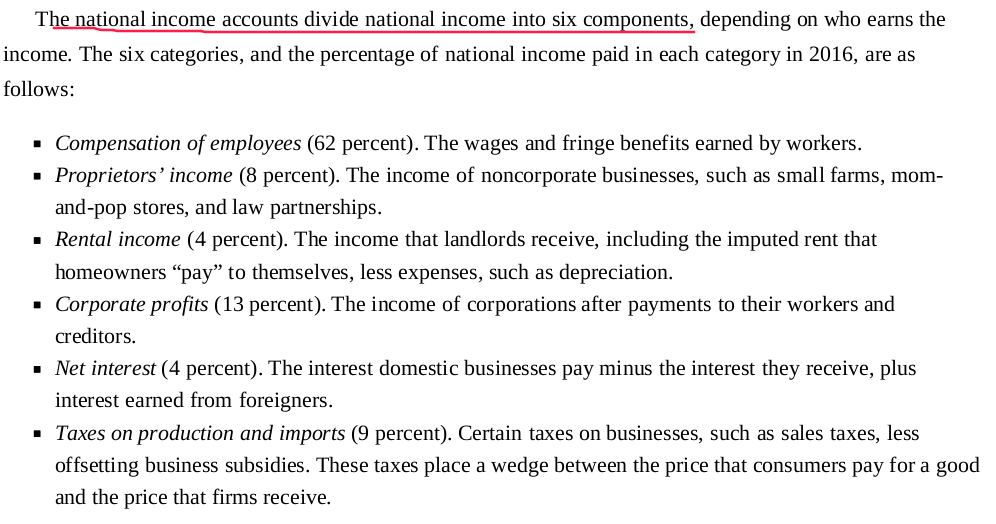
\includegraphics[scale =.5 ]  {figures/six_components_of_national_income.png}}
\end{figure}


\subsubsection{Personal Income}
A series of adjustments take us from national income to personal income, the amount of 
income that households and noncorporate businesses receive.

\begin{figure}[H]
\center{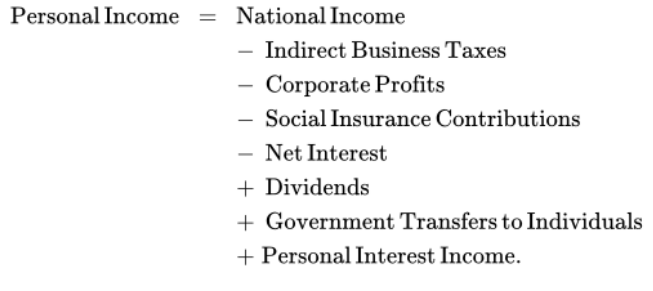
\includegraphics[scale =.5 ]  {figures/personal_income.png}}
\end{figure}

Indirect Business Taxes: we subtract taxes on production and imports because these taxes
never enter anyone’s income.









%\bibliographystyle{plainnat}
%\bibliography{my_bib}

\end{document}

